%In this section you will discuss the Technical Development related to your project.
%In one or more chapters you must describe fully the design and development strategies you have adopted and the results achieved.  You may refer to appropriate User and System documentation presented as appendices to avoid repeating extensive detail, so you can focus here instead on a discussion of your reasons for adopting the techniques and strategies you have followed.
%Again, it is difficult to give prescriptive guidance on the subsection structure you might adopt, as this will depend on the nature and content of your project.  However, you will probably want at least to consider sections addressing issues of System Design; Implementation; Testing.  If there is a lot to cover in any of these areas, it may warrant presentation as a full chapter rather than a section.
\chapter{Technical Development}

\section{Overview}

\subsection{Script Design}
The script utilises a section in the Linux kernel refereed to as the ``NFQUEUE''. This is as the name suggests a queue that is stored in kernel memory that will store up packets until the user provides one of the two verdicts: `Drop' or `Accept'. The packets are pushed into this queue by the use of `iptable' rules, iptabales is a tool designed to filter packets by criteria. Below is a flow diagram for the path a packet might take, each table can have filtering rules embedded into to it:

% Diagram
%Variables
\newcommand{\nodefont}{\rmfamily}
\newcommand{\normalWidth}{3cm}

%----------------------------------------%
%  IPtables Diagram						 %
%----------------------------------------%
\tikzset{%
  >={Latex[width=2mm,length=2mm]},
  % Specifications for style of nodes:
            base/.style = {rectangle, rounded corners, draw=black,
                           minimum width=4cm, minimum height=1cm,
                           text centered, font=\sffamily}, 
            process/.style = {base, minimum width=\normalWidth, fill=orange!15,
                           font=\nodefont},
            network/.style = {base, fill=blue!15},
            local/.style = {base, fill=red!15}}
\vspace{0.25cm}                
\begin{center}
\begin{tikzpicture}[node distance=1.5cm, every node/.style={fill=white, font=\sffamily}, align=center]
    	\node(NetworkCard)[network]{Network Card};
        \node(NetworkCardOut)[network, right of=NetworkCard, xshift=6cm]{Network Card};
        
    	\node(PreRouting)[process, below of=NetworkCard]{Pre-Routing};
    	\node(Forward)[process, right of=PreRouting, xshift=2.5cm, yshift=-1.75cm]{Forward};
    	\node(Input)[process, below of=PreRouting, yshift=-2cm]{Input};
        \node(PostRouting)[process, right of=PreRouting, xshift=6cm]{Post-Routing};
    	\node(Output)[process, right of=Input, xshift=6cm]{Output};
        
        \node(LocalProcessIn)[local, below of=Input]{Local Process};
        \node(LocalProcessOut)[local, below of=Output]{Local Process};
        
        %In Arrows
        \draw[->] (NetworkCard)--(PreRouting);
        \draw[->] (PreRouting)|-(Forward);
        \draw[->] (PreRouting)--(Input);
        \draw[->] (Input)--(LocalProcessIn);
        
        %Out Arrows
        \draw[->] (LocalProcessOut)--(Output);
        \draw[->] (Output)--(PostRouting);
        \draw[->] (Forward)-|(PostRouting);
        \draw[->] (PostRouting)--(NetworkCardOut);        
\end{tikzpicture}
\end{center}   

If there was a case where all packets entering the machine need filtering, an iptable rule would be added to the "Pre-Routing" section of the table to catch all packets leaving the machine. 

So for example to move all packets entering from the network card into the NFQUEUE the iptable rule would be added like so:
\begin{center}
	\begin{console_font}
		\large{iptables -A INPUT -j NFQUEUE}
	\end{console_font} 
\end{center}
Where `-a' tells to append a rule onto the `INPUT' table and `-j' is the rule that affects the packet, in this case pushing it into the default queue.

This forms the main component of the functionality of the script, a series of iptable rules that filter packets into the NFQUEUE and allow to script to perform verdicts on each packet separately allows for effects to be easily applied to packets entering and leaving the machine.

\subsection{Degradation Effects}
The script contains the functionality to simulate a plethora of effects each one and its functionality will be described below. Please not any of these effects can be chained together in any order.

\subsubsection*{Latency}
Latency as described in the background section is the delay in initiating a task and seeing its results. Latency is simulated by using a timing mechanisms where the arrival time of the packet is saved. The packet is then pushed into the NFQUEUE that triggers a single thread that will hold the packet for a set amount of time, the holding time is calculated by taking the amount of time the packet has already been in the script away from the target time. The packet is then marked as `ACCEPTED' and pushed out of the queue.

\subsubsection*{Packet Loss}
Packet loss is simulated by first assigning a target value, lets say for this example 10\%. For each packet the script randomly generates a number between 1 and 100, if that value is less than the target value the packet is dropped, and if the value is larger the packet is accepted. This therefore creates the effect of packet loss. It does however require a fair amount of packets to balance out statistically and reach the percentage target.

\subsubsection*{Bandwidth}
There are two modes created for bandwidth; rate limiting and a simple display. Rate limiting allows the script to limit the rate of bandwidth flowing through the machine and calculates the rate transferred over a period of 5 seconds, if the rate is higher it waits until the rate drops below the target. This gives it the ability to adjust quickly and allows the script to be run for a long period of time without the overall average of the bandwidth affecting future changes. Displaying the bandwidth work exactly the same but without the limit check, this is useful when checking the current download speeds or the max transfer rate.

\subsubsection*{Out-of-order}
This effect changes the order of packets coming into the script, this can be used to check its effect on UDP and TCP and can test how quickly these issue can be rectified. It works by queuing up every packet into a list, then a single thread randomly picks an index of that list, accepts the packet and allows it to leave this means at its most extreme the order can be last in, first out and therefore going against normal operation.

\subsubsection*{Connection Simulation}
Connection simulation isn't quite a degradation effect but its intent is to simulate the effect of degradation on a common connection like `WiFi` or a 3G connection to see how these connections are effected by said degradation. This can be useful in some situations where for example testing a mobile applications performance over 3G with heavy latency, the mobile would connect to the script and the script would effect any traffic entering or leaving the handset.

\subsubsection*{Jitter}
Jitter mode clumps and separates packets in their transmission, with some it waits a small period of time other it will clump up delay as a total and then send them all at once. This is to test how the protocol deals with jitter in the connection. Jitter as explained in the background is the intra-packet latency i.e. the difference in time between arrivals of packets.

\subsection{ARP Spoofing}
The script also supports an ARP spoofing mode that allows it to sit between a gateway and a specified target. This means the script can perform all its functions on a single target with a very quick deployment time. As touched on in the background the ARP protocol performs no authentication on any changes to the ARP cache meaning that you can perform a man in the middle attack and route traffic through a machine of your choice.

The script begins by grabbing the MAC addresses connected to the provided gateway and target IP addresses. Two ARP reply packets (denote by the `2' opcode) are sent out: One telling the victim that the current machines MAC address maps to the gateway, and the other telling the gateway that the victims IP maps to the current machines MAC address.

Below is the process visualised:

\newcommand{\cisco}{cisco_images}
\newcommand{\scale}{0.7}

% Gateway
\newcommand{\GatewayLabel}{
\begin{tabular}{l l}
Gateway\\
\hline
\vspace{0.1cm}
\bf{192.168.1.1} & \bf{C8:49:BD:82:47:4D}\\
ARP Cache\\
\hline
192.168.1.2 & 46:41:73:EC:70:E3
\end{tabular}
}

%Victim
\newcommand{\VictimLabel}{
\begin{tabular}{l l}
Victim\\
\hline
\vspace{0.1cm}
\bf{192.168.1.2} & \bf{46:41:73:EC:70:E3}\\
ARP Cache\\
\hline
192.168.1.1 & C8:49:BD:82:47:4D
\end{tabular}
}

\begin{center}
\begin{tikzpicture}[
    diagram item/.style={},
    align=left
]         

\node (Router)[
    diagram item,
    label=above:\GatewayLabel,
    yshift=-2cm
] {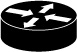
\includegraphics[scale=\scale]{\cisco/router}};

\node (Victim)[
	diagram item,
	label=above:\VictimLabel,
	right of=Router,
	xshift=7cm
] {
\includegraphics[scale=\scale]{\cisco/workstation}};


\draw[-] (Router)--(Victim);

\end{tikzpicture} 
\end{center}


As you can see both ends are connected and have gone through the process to resolve the IP addresses to MAC addresses, you can see above each device their corresponding IP, MAC and ARP Cache. The ARP cache as mentioned previously is a record linking IP addresses to MAC addresses.

\newcommand{\tgap}{0.1cm}

% Gateway
\newcommand{\GatewayLabelAfter}{
\begin{tabular}{l l}
Gateway\\
\hline
\vspace{\tgap}
\bf{192.168.1.1} & \bf{C8:49:BD:82:47:4D}\\
ARP Cache\\
\hline
192.168.1.2 & \bf{\textcolor{red}{37:A8:22:F6:BB:34}} \\
192.168.1.3 & 37:A8:22:F6:BB:34
\end{tabular}
}

%Victim
\newcommand{\VictimLabelAfter}{
\begin{tabular}{l l}
Victim\\
\hline
\vspace{\tgap}
\bf{192.168.1.2} & \bf{46:41:73:EC:70:E3}\\
ARP Cache\\
\hline
192.168.1.1 & \bf{\textcolor{red}{37:A8:22:F6:BB:34}} \\
192.168.1.3 & 37:A8:22:F6:BB:34
\end{tabular}
}

%Attacker
\newcommand{\AttackerLabel}{
\begin{tabular}{l l}
Attacker\\
\hline
\bf{192.168.1.3} & \bf{37:A8:22:F6:BB:34} 
\end{tabular}
}

\begin{center}
\begin{tikzpicture}[
    diagram item/.style={},
    align=left
]         

\node (Router)[
    diagram item,
    label=above:\GatewayLabelAfter,
    yshift=-2cm
] {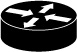
\includegraphics[scale=\scale]{\cisco/router}};

\node (Victim)[
	diagram item,
	label=above:\VictimLabelAfter,
	right of=Router,
	xshift=7cm
] {
\includegraphics[scale=\scale]{\cisco/workstation}};

\node (Attacker)[
	label=below:\AttackerLabel,
	below of=Victim,
	xshift=-3.5cm,
	yshift=-3.5cm
] {
\includegraphics[scale=\scale]{\cisco/laptop}};

\draw[red, very thick] (Router)--(Attacker);
\draw[red, very thick] (Attacker)--(Victim);


\end{tikzpicture} 
\end{center}


Note after the 3rd device connects to the network, both devices gain a record of its IP and MAC address in their ARP cache. 

After both spoofed packets have been send out the ARP cache for each receiving end gets updated, the text in red shows the changes caused by the spoofed ARP packets. Now when either end wants to talk to each other it will resolve the MAC address and send it with the new MAC address in the table, this will therefore get routed through the attacking PC and will allow the script to receive all the traffic between the two parties.

\subsection{Network Attacks}
A couple of network attacks were implemented into the script, these served the purpose of providing very heavy artificial traffic designed to create heavy loads or mess with integral protocols. Not many attacks were added as they don't provide much purpose apart from stress testing and they're on the edge of the scope of this project. There will also be a brief discussion into possible techniques to mitigate the effects. 

\subsubsection{UDP Flooding}
UDP flooding is a very simple attack, lots and lots of UDP packets are created and send over a network stream very quickly. This attack is designed to `flood' the buffers in the receiving machine and slow down or event prevent internet connection. The script creates 10 or so threads that create and send packet concurrently, this amount of threads easily reaches the max throughput of the test machines NIC card and massively reduces internet connection of the receiving end.

The attack could be detected and prevented by a script that monitors the network transfers rates, this attack will create a huge spike in the transfer rate that can be detected and all traffic would be blocked from the sending party.

\subsubsection{ARP Spamming}
This attack works by once again exploiting the lack of authentication of the ARP protocol. In the entire network mode the script starts by detecting all active hosts on a network, it then starts sending out falsified ARP reply packets with randomly generated MAC addresses inside. This results in all computer on the networking having incorrect ARP cache values and resulting in computers incorrectly resolving IP and MAC address combinations and traffic not being allowed through.

This attack is relatively easy to execute but can simply be prevented by issuing static ARP tables for each machine, this prevents unsolicited ARP replies from changing IP and MAC address combinations and also prevents ARP Spoofing from occurring on that network.

%System design:
%This can include UML diagrams such as class diagrams, use case diagrams, activity diagrams, etc.
%If you find that these are taking up a lot of space/words, then you should prioritise and relegate where appropriate to the appendices. 
%This should not just be a list of unexplained diagrams, but should rather include discussions of the most interesting parts of your design, tying them to your background and objectives.
\section{System design}



%UI design:%
%If your software includes user interaction then you could also include a discussion (supported by diagrams) of decisions that you have made regarding the user interface.%
\section{UI design}



%Experimental design:
%If you project includes any experiments, including but not limited to user testing, then you can discuss their design here. Note that again this does not exist in a vacuum and should be tied to your research.
\section{Experiential design}

\subsubsection{Packet Loss and its effect on download speeds}

% Better graph needed
\begin{center}
	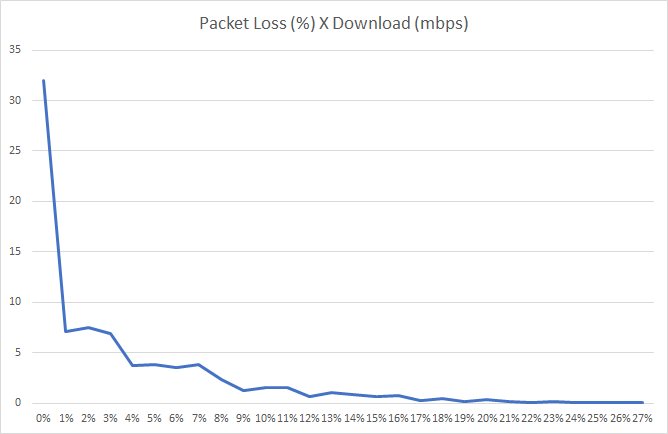
\includegraphics[scale=0.6]{PL_Download}
	\begin{figure}[h]
	 	\caption{Graph displaying effect of packet loss on download speeds}
	\end{figure}		
\end{center}

The graph above shows the download speed measured in Mbps against the increasing rate of packet loss, as you can see the download rate only reaches 28\%, this is due to the connection test failing at anything above. The tests were performed by querying the SpeedTest.net \comments{CITE} API. 

My initial hypothesis for the sharp decreases in packet loss from 0\% to 1\% is it's due to the congestion control mechanisms built into TCP. TCP as mentioned in the background section allows for multiple devices to co-exist on a network and dynamically balance network resources through congestion control algorithms, but packet loss in this aspect is assumed as a sign of congestion to the algorithm adapts and reduces its transfer rate each time a packet is lost, this means the transfer rate drastically reduces until it reaches a platform.

%The test for this will check the transfer rate over a period of time where it will drop a packet every 10 seconds and hopefully will see a dip in transfer rate when each packet is dropped

\comments{Decide on an experiment to prove this}
\comments{Also talk about why the transfer fails when the packet loss reaches 28\%}

\subsubsection{Latency and retransmission}

\comments{Graph here showing linear retransmission against increasing latency value}
The expected result from this graph was a large peak at the time out period where all the packets send would flag up as retransmissions. This graph is flat due to the dynamic way that TCP works out its RTO (Retransmission Timeout) value that includes the Round trip time (i.e) and this test that created the graph above has the latency affecting the entire time to the dynamic value of the RTO was using the latency value to calculate it and therefore meant that changing the value of latency had no effect 

% ## Reading
% https://tools.ietf.org/html/rfc6298
% https://sgros.blogspot.co.uk/2012/02/calculating-tcp-rto.html
% https://blog.catchpoint.com/2014/04/29/understanding-rtt-impact-on-tcp-retransmissions/

% Maybe a test where the handshake has not latency on it?
% Then the latency is increased to a cetain value 

\comments{Changing value of latency won't ever stop a TCP connection??}


%Test design and system testing:
%Testing is an extremely important part of any software project and should not be a tacked on afterthought. You can include here a discussion of the design of any tests that you intend to carry out on your project. It would not be appropriate to include an exhaustive list of all the individual tests that you wish to conduct (consider the appendices for this) but examples would be useful to illustrate your discussion.
%You should review how you have approached the testing and quality assurance of your delivered product, including relevant choice of incremental and/or integration testing, test scenarios, sample datasets, etc. as appropriate,  Exhaustive reproduction of extensive test records is not required, but sample evidence should be used to support your discussion.
\section{Test design and system testing}



%System Implementation:$
%You should review how you have implemented your project system, discussing any areas of the implementation which might for example involve code or processes which are not immediately obvious in structure or operation, where you have had to innovate or develop particular approaches.  Again, you should refer to relevant diagrams of code or object structures which should be included in documentation as appended.
\section{System Implementation}

